\documentclass[10pt,a4paper]{article} % Prepara un documento con un font grande

\input{./preamboli_e_stili/pacchetti.tex}

\DeclareGraphicsExtensions{.pdf, .png, .jpg} % Se due immagini hanno lo stesso nome sceglile secondo l'ordine di filetype qui
\graphicspath{ {./img/} }					 % Path delle immagini 

\input{./preamboli_e_stili/titolo_Calorimetro.tex}
\input{./preamboli_e_stili/stili_float.tex}


%////////////////////////////////////////////////////////////////////////////////////////////////////////////////////////////
%////////////////////////////////////////////////////////////////////////////////////////////////////////////////////////////
% Fine dei dati iniziali per il latex: il documento finale inizierà da qui
\begin{document}

\maketitle % Produce il titolo a partire dai comandi \title, \author e \date

\vspace{15mm}
\begin{center}
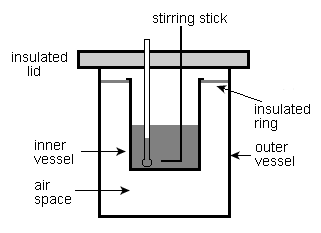
\includegraphics[width=0.6\textwidth]{calorimeter}
\end{center}

\vfill
% Le varie sezioni
%\section{Obiettivi}
\begin{abstract}
	\noindent
	Sima del calore specifico di un corpo.
Riconoscimento del materiale di un corpo attraverso il confronto del suo calore specifico con le tabelle fornite.


\end{abstract}

\newpage

\tableofcontents % Prepara l'indice generale

%\begin{multicols}{2}

\section{Apparato strumentale}
	


\section{Metodologia di misura}
	Per poter raggiungere gli obiettivi prefissati, si è ripetuto l’esperimento nella sua interezza più volte. L’esperimento è stato suddiviso 
in fasi successive per un’ottimizzazione dei risultati e del tempo impiegato.
\begin{description}

  \item[Fase 1] \hfill \\
	  Misurazione delle masse: per prima cosa si sono misurate sulla bilancia di precisione le masse che venivano inserite all’interno 
	  del calorimetro: il recipiente per l’acqua assieme all’agitatore e il cilindro in acciaio. Successivamente è stato riempito il 
	  contenitore con dell’acqua sufficiente a permettere l’immersione totale del cilindro, ed il sistema recipiente-agitatore-acqua è 
	  stato nuovamente pesato per avere una stima della massa dell’acqua utilizzata.
  \item[Fase 2] \hfill \\
	  Preparazione: per preparare l’esperimento per prima cosa si è messo il cilindro a riscaldare nello strumento apposito, dopodiché 
	  si è posto nel calorimetro il recipiente con l’acqua, si è bloccato il coperchio, avvitato l’agitatore al supporto presente sul 
	  tappo del calorimetro, e si e immerso in acqua il termometro (sempre attraverso l’apposito supporto).
  \item[Fase 3] \hfill \\
	Misurazione dei tempi: non appena il riscaldatore ha portato il cilindro a 
	temperatura (valore che dipendeva, di volta in volta, a causa delle condizioni del riscaldatore e delle condizioni ambientali e fluttuazioni casuali), 
	si è agitata l’acqua grazie all’agitatore, e registrata la misura della temperatura mostrata dal termometro immerso in acqua. 
	Successivamente, il più rapidamente possibile, si è preso il cilindro grazie al filo a cui era attaccato e si è immerso nell’acqua
	posta dentro il calorimetro facendolo passare dall’apposito buco, repentinamente chiuso. Un altro sperimentatore ha cercato con 
	maggior precisione possibile di avviare il cronometro nel momento in cui il cilindro si è immerso in acqua. Per limitare gli errori
	di zero il movimento dello sperimentatore che ha spostato il cilindro in acciaio è stato composto di gesti ampi e quindi 
	prevedibile per il secondo sperimentatore, che ha cercato nel miglior modo possibile di riconoscere, nonostante l’assenza del 
	contatto visivo diretto, il momento in cui il cilindro si immergeva in acqua. A intervalli regolari ($5.0 \pm 0.1 $) $s$ è stata 
	registrata la temperatura mostrata dal cronometro immerso in acqua, fino al momento in cui essa non è risultata stabile nel tempo.
	A quel punto si è misurato il tempo segnato dal cronometro durante il cambio della temperatura mostrata dal termometro (secondo la 
	sua scala di riferimento, quindi ogni $0.1 \gradi C$). Preso un numero di misurazioni ritenuto sufficiente si è interrotto l’esperimento 
	aprendo il calorimetro. L’acqua è stata buttata, tutti i componenti sono stati asciugati e si è ripetuto l’esperimento dalla Fase 
	1.
\end{description}



\newpage
\section{Presentazione dei dati}			
	\subsection{Tabelle}
	\begin{multicols}{2}
	%\begin{tabella}
%	\centering
%	\input{./tabelle/2030d.tex}
%	\caption{Periodo di oscillazione [s] in posizione dritta, intervalli di 2cm}
%	\label{tab:dec}
%\end{tabella}


	\end{multicols}
	\clearpage
	\subsection{Grafici}
	%\begin{grafico}
%    \centering
%\input{../gnuplot/immagini/parabola.tex}
%\caption{Rami di parabola contenenti le due intersezioni}
%\label{img:dec}
%\end{grafico}

\begin{grafico}
    \centering
\begin{tikzpicture}[gnuplot]
%% generated with GNUPLOT 4.6p3 (Lua 5.1; terminal rev. 99, script rev. 100)
%% mar 13 mag 2014 17:23:06 CEST
\gpmonochromelines
\path (0.000,0.000) rectangle (12.500,8.750);
\gpcolor{color=gp lt color border}
\gpsetlinetype{gp lt border}
\gpsetlinewidth{1.00}
\draw[gp path] (1.320,0.985)--(1.500,0.985);
\draw[gp path] (11.947,0.985)--(11.767,0.985);
\node[gp node right] at (1.136,0.985) { 23};
\draw[gp path] (1.320,2.125)--(1.500,2.125);
\draw[gp path] (11.947,2.125)--(11.767,2.125);
\node[gp node right] at (1.136,2.125) { 24};
\draw[gp path] (1.320,3.265)--(1.500,3.265);
\draw[gp path] (11.947,3.265)--(11.767,3.265);
\node[gp node right] at (1.136,3.265) { 25};
\draw[gp path] (1.320,4.405)--(1.500,4.405);
\draw[gp path] (11.947,4.405)--(11.767,4.405);
\node[gp node right] at (1.136,4.405) { 26};
\draw[gp path] (1.320,5.545)--(1.500,5.545);
\draw[gp path] (11.947,5.545)--(11.767,5.545);
\node[gp node right] at (1.136,5.545) { 27};
\draw[gp path] (1.320,6.685)--(1.500,6.685);
\draw[gp path] (11.947,6.685)--(11.767,6.685);
\node[gp node right] at (1.136,6.685) { 28};
\draw[gp path] (1.320,7.825)--(1.500,7.825);
\draw[gp path] (11.947,7.825)--(11.767,7.825);
\node[gp node right] at (1.136,7.825) { 29};
\draw[gp path] (1.320,0.985)--(1.320,1.165);
\draw[gp path] (1.320,7.825)--(1.320,7.645);
\node[gp node center] at (1.320,0.677) { 0};
\draw[gp path] (3.445,0.985)--(3.445,1.165);
\draw[gp path] (3.445,7.825)--(3.445,7.645);
\node[gp node center] at (3.445,0.677) { 50};
\draw[gp path] (5.571,0.985)--(5.571,1.165);
\draw[gp path] (5.571,7.825)--(5.571,7.645);
\node[gp node center] at (5.571,0.677) { 100};
\draw[gp path] (7.696,0.985)--(7.696,1.165);
\draw[gp path] (7.696,7.825)--(7.696,7.645);
\node[gp node center] at (7.696,0.677) { 150};
\draw[gp path] (9.822,0.985)--(9.822,1.165);
\draw[gp path] (9.822,7.825)--(9.822,7.645);
\node[gp node center] at (9.822,0.677) { 200};
\draw[gp path] (11.947,0.985)--(11.947,1.165);
\draw[gp path] (11.947,7.825)--(11.947,7.645);
\node[gp node center] at (11.947,0.677) { 250};
\draw[gp path] (1.320,7.825)--(1.320,0.985)--(11.947,0.985)--(11.947,7.825)--cycle;
\node[gp node center,rotate=-270] at (0.246,4.405) {Temperatura $[\gradi C]$};
\node[gp node center] at (6.633,0.215) {Tempo $[s]$};
\node[gp node center] at (6.633,8.287) {Test 1};
\node[gp node left] at (3.855,1.627) {Dati};
\gpcolor{color=gp lt color 0}
\gpsetpointsize{4.00}
\gppoint{gp mark 1}{(1.533,1.441)}
\gppoint{gp mark 1}{(1.745,4.291)}
\gppoint{gp mark 1}{(1.958,6.229)}
\gppoint{gp mark 1}{(2.170,6.913)}
\gppoint{gp mark 1}{(2.383,7.369)}
\gppoint{gp mark 1}{(2.595,7.483)}
\gppoint{gp mark 1}{(2.808,7.597)}
\gppoint{gp mark 1}{(3.020,7.597)}
\gppoint{gp mark 1}{(3.233,7.597)}
\gppoint{gp mark 1}{(3.445,7.711)}
\gppoint{gp mark 1}{(5.401,7.597)}
\gppoint{gp mark 1}{(7.994,7.483)}
\gppoint{gp mark 1}{(11.437,7.369)}
\gppoint{gp mark 1}{(11.121,1.627)}
\gpcolor{color=gp lt color border}
\node[gp node left] at (3.855,1.319) {Perdita di calore: $f(x) = a[\gradi C] + b [\frac{\gradi C}{s}] \cdot x$};
\gpcolor{color=gp lt color 1}
\gpsetlinetype{gp lt plot 1}
\draw[gp path] (10.663,1.319)--(11.579,1.319);
\draw[gp path] (1.533,7.492)--(1.633,7.491)--(1.733,7.489)--(1.833,7.488)--(1.933,7.487)%
  --(2.033,7.486)--(2.133,7.484)--(2.233,7.483)--(2.333,7.482)--(2.433,7.481)--(2.533,7.479)%
  --(2.633,7.478)--(2.733,7.477)--(2.833,7.476)--(2.933,7.474)--(3.033,7.473)--(3.133,7.472)%
  --(3.233,7.471)--(3.333,7.470)--(3.433,7.468)--(3.533,7.467)--(3.633,7.466)--(3.734,7.465)%
  --(3.834,7.463)--(3.934,7.462)--(4.034,7.461)--(4.134,7.460)--(4.234,7.458)--(4.334,7.457)%
  --(4.434,7.456)--(4.534,7.455)--(4.634,7.454)--(4.734,7.452)--(4.834,7.451)--(4.934,7.450)%
  --(5.034,7.449)--(5.134,7.447)--(5.234,7.446)--(5.334,7.445)--(5.434,7.444)--(5.534,7.442)%
  --(5.634,7.441)--(5.734,7.440)--(5.834,7.439)--(5.934,7.437)--(6.035,7.436)--(6.135,7.435)%
  --(6.235,7.434)--(6.335,7.433)--(6.435,7.431)--(6.535,7.430)--(6.635,7.429)--(6.735,7.428)%
  --(6.835,7.426)--(6.935,7.425)--(7.035,7.424)--(7.135,7.423)--(7.235,7.421)--(7.335,7.420)%
  --(7.435,7.419)--(7.535,7.418)--(7.635,7.416)--(7.735,7.415)--(7.835,7.414)--(7.935,7.413)%
  --(8.035,7.412)--(8.135,7.410)--(8.235,7.409)--(8.336,7.408)--(8.436,7.407)--(8.536,7.405)%
  --(8.636,7.404)--(8.736,7.403)--(8.836,7.402)--(8.936,7.400)--(9.036,7.399)--(9.136,7.398)%
  --(9.236,7.397)--(9.336,7.396)--(9.436,7.394)--(9.536,7.393)--(9.636,7.392)--(9.736,7.391)%
  --(9.836,7.389)--(9.936,7.388)--(10.036,7.387)--(10.136,7.386)--(10.236,7.384)--(10.336,7.383)%
  --(10.436,7.382)--(10.537,7.381)--(10.637,7.379)--(10.737,7.378)--(10.837,7.377)--(10.937,7.376)%
  --(11.037,7.375)--(11.137,7.373)--(11.237,7.372)--(11.337,7.371)--(11.437,7.370);
\gpcolor{color=gp lt color border}
\gpsetlinetype{gp lt border}
\draw[gp path] (1.320,7.825)--(1.320,0.985)--(11.947,0.985)--(11.947,7.825)--cycle;
%% coordinates of the plot area
\gpdefrectangularnode{gp plot 1}{\pgfpoint{1.320cm}{0.985cm}}{\pgfpoint{11.947cm}{7.825cm}}
\end{tikzpicture}
%% gnuplot variables

\caption{Primo Test: $\quad y = (28.71 \pm 0.01) + (-0.00046 \pm 0.00003) x$}
\label{img:t1}
\end{grafico}

%\[ y = (28.71 \pm 0.01) + (-0.00046 \pm 0.00003) x\]

\begin{grafico}
    \centering
\begin{tikzpicture}[gnuplot]
%% generated with GNUPLOT 4.6p3 (Lua 5.1; terminal rev. 99, script rev. 100)
%% mar 13 mag 2014 17:23:06 CEST
\gpmonochromelines
\path (0.000,0.000) rectangle (12.500,8.750);
\gpcolor{color=gp lt color border}
\gpsetlinetype{gp lt border}
\gpsetlinewidth{1.00}
\draw[gp path] (1.320,0.985)--(1.500,0.985);
\draw[gp path] (11.947,0.985)--(11.767,0.985);
\node[gp node right] at (1.136,0.985) { 22};
\draw[gp path] (1.320,2.125)--(1.500,2.125);
\draw[gp path] (11.947,2.125)--(11.767,2.125);
\node[gp node right] at (1.136,2.125) { 23};
\draw[gp path] (1.320,3.265)--(1.500,3.265);
\draw[gp path] (11.947,3.265)--(11.767,3.265);
\node[gp node right] at (1.136,3.265) { 24};
\draw[gp path] (1.320,4.405)--(1.500,4.405);
\draw[gp path] (11.947,4.405)--(11.767,4.405);
\node[gp node right] at (1.136,4.405) { 25};
\draw[gp path] (1.320,5.545)--(1.500,5.545);
\draw[gp path] (11.947,5.545)--(11.767,5.545);
\node[gp node right] at (1.136,5.545) { 26};
\draw[gp path] (1.320,6.685)--(1.500,6.685);
\draw[gp path] (11.947,6.685)--(11.767,6.685);
\node[gp node right] at (1.136,6.685) { 27};
\draw[gp path] (1.320,7.825)--(1.500,7.825);
\draw[gp path] (11.947,7.825)--(11.767,7.825);
\node[gp node right] at (1.136,7.825) { 28};
\draw[gp path] (1.320,0.985)--(1.320,1.165);
\draw[gp path] (1.320,7.825)--(1.320,7.645);
\node[gp node center] at (1.320,0.677) { 0};
\draw[gp path] (2.838,0.985)--(2.838,1.165);
\draw[gp path] (2.838,7.825)--(2.838,7.645);
\node[gp node center] at (2.838,0.677) { 50};
\draw[gp path] (4.356,0.985)--(4.356,1.165);
\draw[gp path] (4.356,7.825)--(4.356,7.645);
\node[gp node center] at (4.356,0.677) { 100};
\draw[gp path] (5.874,0.985)--(5.874,1.165);
\draw[gp path] (5.874,7.825)--(5.874,7.645);
\node[gp node center] at (5.874,0.677) { 150};
\draw[gp path] (7.393,0.985)--(7.393,1.165);
\draw[gp path] (7.393,7.825)--(7.393,7.645);
\node[gp node center] at (7.393,0.677) { 200};
\draw[gp path] (8.911,0.985)--(8.911,1.165);
\draw[gp path] (8.911,7.825)--(8.911,7.645);
\node[gp node center] at (8.911,0.677) { 250};
\draw[gp path] (10.429,0.985)--(10.429,1.165);
\draw[gp path] (10.429,7.825)--(10.429,7.645);
\node[gp node center] at (10.429,0.677) { 300};
\draw[gp path] (11.947,0.985)--(11.947,1.165);
\draw[gp path] (11.947,7.825)--(11.947,7.645);
\node[gp node center] at (11.947,0.677) { 350};
\draw[gp path] (1.320,7.825)--(1.320,0.985)--(11.947,0.985)--(11.947,7.825)--cycle;
\node[gp node center,rotate=-270] at (0.246,4.405) {Temperatura $[\gradi C]$};
\node[gp node center] at (6.633,0.215) {Tempo $[s]$};
\node[gp node center] at (6.633,8.287) {Test 2};
\node[gp node left] at (3.855,1.627) {Dati};
\gpcolor{color=gp lt color 0}
\gpsetpointsize{4.00}
\gppoint{gp mark 1}{(1.472,1.555)}
\gppoint{gp mark 1}{(1.624,3.835)}
\gppoint{gp mark 1}{(1.775,5.431)}
\gppoint{gp mark 1}{(1.927,6.229)}
\gppoint{gp mark 1}{(2.079,6.571)}
\gppoint{gp mark 1}{(2.231,7.255)}
\gppoint{gp mark 1}{(2.383,7.369)}
\gppoint{gp mark 1}{(2.535,7.483)}
\gppoint{gp mark 1}{(2.686,7.597)}
\gppoint{gp mark 1}{(2.838,7.711)}
\gppoint{gp mark 1}{(6.603,7.597)}
\gppoint{gp mark 1}{(9.093,7.483)}
\gppoint{gp mark 1}{(11.704,7.369)}
\gppoint{gp mark 1}{(11.121,1.627)}
\gpcolor{color=gp lt color border}
\node[gp node left] at (3.855,1.319) {Perdita di calore: $f(x) = a[\gradi C] + b [\frac{\gradi C}{s}] \cdot x$};
\gpcolor{color=gp lt color 1}
\gpsetlinetype{gp lt plot 1}
\draw[gp path] (10.663,1.319)--(11.579,1.319);
\draw[gp path] (1.472,7.774)--(1.575,7.770)--(1.679,7.766)--(1.782,7.762)--(1.885,7.758)%
  --(1.989,7.754)--(2.092,7.750)--(2.195,7.746)--(2.299,7.742)--(2.402,7.738)--(2.505,7.734)%
  --(2.609,7.730)--(2.712,7.726)--(2.815,7.722)--(2.919,7.718)--(3.022,7.714)--(3.126,7.710)%
  --(3.229,7.706)--(3.332,7.702)--(3.436,7.698)--(3.539,7.694)--(3.642,7.690)--(3.746,7.686)%
  --(3.849,7.682)--(3.952,7.678)--(4.056,7.674)--(4.159,7.670)--(4.262,7.666)--(4.366,7.662)%
  --(4.469,7.658)--(4.573,7.654)--(4.676,7.650)--(4.779,7.646)--(4.883,7.642)--(4.986,7.638)%
  --(5.089,7.634)--(5.193,7.630)--(5.296,7.626)--(5.399,7.622)--(5.503,7.618)--(5.606,7.614)%
  --(5.709,7.610)--(5.813,7.606)--(5.916,7.602)--(6.019,7.598)--(6.123,7.594)--(6.226,7.590)%
  --(6.330,7.586)--(6.433,7.582)--(6.536,7.578)--(6.640,7.574)--(6.743,7.570)--(6.846,7.566)%
  --(6.950,7.562)--(7.053,7.558)--(7.156,7.554)--(7.260,7.550)--(7.363,7.546)--(7.466,7.542)%
  --(7.570,7.538)--(7.673,7.534)--(7.777,7.530)--(7.880,7.526)--(7.983,7.522)--(8.087,7.518)%
  --(8.190,7.514)--(8.293,7.510)--(8.397,7.506)--(8.500,7.502)--(8.603,7.498)--(8.707,7.494)%
  --(8.810,7.490)--(8.913,7.486)--(9.017,7.482)--(9.120,7.478)--(9.224,7.474)--(9.327,7.470)%
  --(9.430,7.466)--(9.534,7.462)--(9.637,7.458)--(9.740,7.454)--(9.844,7.450)--(9.947,7.446)%
  --(10.050,7.442)--(10.154,7.438)--(10.257,7.434)--(10.360,7.430)--(10.464,7.426)--(10.567,7.422)%
  --(10.671,7.418)--(10.774,7.414)--(10.877,7.410)--(10.981,7.406)--(11.084,7.402)--(11.187,7.398)%
  --(11.291,7.394)--(11.394,7.390)--(11.497,7.386)--(11.601,7.382)--(11.704,7.378);
\gpcolor{color=gp lt color border}
\gpsetlinetype{gp lt border}
\draw[gp path] (1.320,7.825)--(1.320,0.985)--(11.947,0.985)--(11.947,7.825)--cycle;
%% coordinates of the plot area
\gpdefrectangularnode{gp plot 1}{\pgfpoint{1.320cm}{0.985cm}}{\pgfpoint{11.947cm}{7.825cm}}
\end{tikzpicture}
%% gnuplot variables

\caption[]{Secondo Test: $\quad y = (27.96 \pm 0.01) + (-0.00103 \pm 0.00007)  x$}
\label{img:t2}
\end{grafico}

\begin{grafico}
    \centering
\begin{tikzpicture}[gnuplot]
%% generated with GNUPLOT 4.6p3 (Lua 5.1; terminal rev. 99, script rev. 100)
%% mar 13 mag 2014 18:41:53 CEST
\gpmonochromelines
\path (0.000,0.000) rectangle (12.500,8.750);
\gpcolor{color=gp lt color border}
\gpsetlinetype{gp lt border}
\gpsetlinewidth{1.00}
\draw[gp path] (1.320,0.985)--(1.500,0.985);
\draw[gp path] (11.947,0.985)--(11.767,0.985);
\node[gp node right] at (1.136,0.985) { 23};
\draw[gp path] (1.320,1.840)--(1.500,1.840);
\draw[gp path] (11.947,1.840)--(11.767,1.840);
\node[gp node right] at (1.136,1.840) { 24};
\draw[gp path] (1.320,2.695)--(1.500,2.695);
\draw[gp path] (11.947,2.695)--(11.767,2.695);
\node[gp node right] at (1.136,2.695) { 25};
\draw[gp path] (1.320,3.550)--(1.500,3.550);
\draw[gp path] (11.947,3.550)--(11.767,3.550);
\node[gp node right] at (1.136,3.550) { 26};
\draw[gp path] (1.320,4.405)--(1.500,4.405);
\draw[gp path] (11.947,4.405)--(11.767,4.405);
\node[gp node right] at (1.136,4.405) { 27};
\draw[gp path] (1.320,5.260)--(1.500,5.260);
\draw[gp path] (11.947,5.260)--(11.767,5.260);
\node[gp node right] at (1.136,5.260) { 28};
\draw[gp path] (1.320,6.115)--(1.500,6.115);
\draw[gp path] (11.947,6.115)--(11.767,6.115);
\node[gp node right] at (1.136,6.115) { 29};
\draw[gp path] (1.320,6.970)--(1.500,6.970);
\draw[gp path] (11.947,6.970)--(11.767,6.970);
\node[gp node right] at (1.136,6.970) { 30};
\draw[gp path] (1.320,7.825)--(1.500,7.825);
\draw[gp path] (11.947,7.825)--(11.767,7.825);
\node[gp node right] at (1.136,7.825) { 31};
\draw[gp path] (1.320,0.985)--(1.320,1.165);
\draw[gp path] (1.320,7.825)--(1.320,7.645);
\node[gp node center] at (1.320,0.677) { 0};
\draw[gp path] (2.648,0.985)--(2.648,1.165);
\draw[gp path] (2.648,7.825)--(2.648,7.645);
\node[gp node center] at (2.648,0.677) { 50};
\draw[gp path] (3.977,0.985)--(3.977,1.165);
\draw[gp path] (3.977,7.825)--(3.977,7.645);
\node[gp node center] at (3.977,0.677) { 100};
\draw[gp path] (5.305,0.985)--(5.305,1.165);
\draw[gp path] (5.305,7.825)--(5.305,7.645);
\node[gp node center] at (5.305,0.677) { 150};
\draw[gp path] (6.634,0.985)--(6.634,1.165);
\draw[gp path] (6.634,7.825)--(6.634,7.645);
\node[gp node center] at (6.634,0.677) { 200};
\draw[gp path] (7.962,0.985)--(7.962,1.165);
\draw[gp path] (7.962,7.825)--(7.962,7.645);
\node[gp node center] at (7.962,0.677) { 250};
\draw[gp path] (9.290,0.985)--(9.290,1.165);
\draw[gp path] (9.290,7.825)--(9.290,7.645);
\node[gp node center] at (9.290,0.677) { 300};
\draw[gp path] (10.619,0.985)--(10.619,1.165);
\draw[gp path] (10.619,7.825)--(10.619,7.645);
\node[gp node center] at (10.619,0.677) { 350};
\draw[gp path] (11.947,0.985)--(11.947,1.165);
\draw[gp path] (11.947,7.825)--(11.947,7.645);
\node[gp node center] at (11.947,0.677) { 400};
\draw[gp path] (1.320,7.825)--(1.320,0.985)--(11.947,0.985)--(11.947,7.825)--cycle;
\node[gp node center,rotate=-270] at (0.246,4.405) {Temperatura $[\gradi C]$};
\node[gp node center] at (6.633,0.215) {Tempo $[s]$};
\node[gp node center] at (6.633,8.287) {Test 3};
\node[gp node left] at (3.855,1.627) {Dati};
\gpcolor{color=gp lt color 0}
\gpsetpointsize{4.00}
\gppoint{gp mark 1}{(1.453,1.413)}
\gppoint{gp mark 1}{(1.586,3.037)}
\gppoint{gp mark 1}{(1.719,3.978)}
\gppoint{gp mark 1}{(1.851,4.918)}
\gppoint{gp mark 1}{(1.984,5.431)}
\gppoint{gp mark 1}{(2.117,5.773)}
\gppoint{gp mark 1}{(2.250,6.029)}
\gppoint{gp mark 1}{(2.383,6.201)}
\gppoint{gp mark 1}{(2.516,6.372)}
\gppoint{gp mark 1}{(2.648,6.543)}
\gppoint{gp mark 1}{(2.781,6.628)}
\gppoint{gp mark 1}{(2.914,6.713)}
\gppoint{gp mark 1}{(3.047,6.713)}
\gppoint{gp mark 1}{(3.180,6.799)}
\gppoint{gp mark 1}{(3.313,6.799)}
\gppoint{gp mark 1}{(3.445,6.799)}
\gppoint{gp mark 1}{(3.578,6.884)}
\gppoint{gp mark 1}{(6.288,6.799)}
\gppoint{gp mark 1}{(7.776,6.713)}
\gppoint{gp mark 1}{(9.343,6.628)}
\gppoint{gp mark 1}{(10.911,6.543)}
\gppoint{gp mark 1}{(11.121,1.627)}
\gpcolor{color=gp lt color border}
\node[gp node left] at (3.855,1.319) {Perdita di calore: $f(x) = a[\gradi C] + b [\frac{\gradi C}{s}] \cdot x$};
\gpcolor{color=gp lt color 1}
\gpsetlinetype{gp lt plot 1}
\draw[gp path] (10.663,1.319)--(11.579,1.319);
\draw[gp path] (1.453,6.998)--(1.548,6.993)--(1.644,6.989)--(1.739,6.984)--(1.835,6.979)%
  --(1.931,6.975)--(2.026,6.970)--(2.122,6.966)--(2.217,6.961)--(2.313,6.956)--(2.408,6.952)%
  --(2.504,6.947)--(2.599,6.942)--(2.695,6.938)--(2.790,6.933)--(2.886,6.929)--(2.981,6.924)%
  --(3.077,6.919)--(3.172,6.915)--(3.268,6.910)--(3.364,6.906)--(3.459,6.901)--(3.555,6.896)%
  --(3.650,6.892)--(3.746,6.887)--(3.841,6.882)--(3.937,6.878)--(4.032,6.873)--(4.128,6.869)%
  --(4.223,6.864)--(4.319,6.859)--(4.414,6.855)--(4.510,6.850)--(4.606,6.846)--(4.701,6.841)%
  --(4.797,6.836)--(4.892,6.832)--(4.988,6.827)--(5.083,6.823)--(5.179,6.818)--(5.274,6.813)%
  --(5.370,6.809)--(5.465,6.804)--(5.561,6.799)--(5.656,6.795)--(5.752,6.790)--(5.847,6.786)%
  --(5.943,6.781)--(6.039,6.776)--(6.134,6.772)--(6.230,6.767)--(6.325,6.763)--(6.421,6.758)%
  --(6.516,6.753)--(6.612,6.749)--(6.707,6.744)--(6.803,6.740)--(6.898,6.735)--(6.994,6.730)%
  --(7.089,6.726)--(7.185,6.721)--(7.281,6.716)--(7.376,6.712)--(7.472,6.707)--(7.567,6.703)%
  --(7.663,6.698)--(7.758,6.693)--(7.854,6.689)--(7.949,6.684)--(8.045,6.680)--(8.140,6.675)%
  --(8.236,6.670)--(8.331,6.666)--(8.427,6.661)--(8.522,6.657)--(8.618,6.652)--(8.714,6.647)%
  --(8.809,6.643)--(8.905,6.638)--(9.000,6.633)--(9.096,6.629)--(9.191,6.624)--(9.287,6.620)%
  --(9.382,6.615)--(9.478,6.610)--(9.573,6.606)--(9.669,6.601)--(9.764,6.597)--(9.860,6.592)%
  --(9.956,6.587)--(10.051,6.583)--(10.147,6.578)--(10.242,6.574)--(10.338,6.569)--(10.433,6.564)%
  --(10.529,6.560)--(10.624,6.555)--(10.720,6.550)--(10.815,6.546)--(10.911,6.541);
\gpcolor{color=gp lt color border}
\gpsetlinetype{gp lt border}
\draw[gp path] (1.320,7.825)--(1.320,0.985)--(11.947,0.985)--(11.947,7.825)--cycle;
%% coordinates of the plot area
\gpdefrectangularnode{gp plot 1}{\pgfpoint{1.320cm}{0.985cm}}{\pgfpoint{11.947cm}{7.825cm}}
\end{tikzpicture}
%% gnuplot variables

\caption[]{Terzo Test: $\quad  y = (30.04 \pm 0.03) + (-0.0015 \pm 0.0001)  x$}
\label{img:t3}
\end{grafico}

\begin{grafico}
    \centering
\begin{tikzpicture}[gnuplot]
%% generated with GNUPLOT 4.6p3 (Lua 5.1; terminal rev. 99, script rev. 100)
%% mar 13 mag 2014 15:56:53 CEST
\gpmonochromelines
\path (0.000,0.000) rectangle (12.500,8.750);
\gpcolor{color=gp lt color border}
\gpsetlinetype{gp lt border}
\gpsetlinewidth{1.00}
\draw[gp path] (1.320,0.985)--(1.500,0.985);
\draw[gp path] (11.947,0.985)--(11.767,0.985);
\node[gp node right] at (1.136,0.985) { 23};
\draw[gp path] (1.320,2.125)--(1.500,2.125);
\draw[gp path] (11.947,2.125)--(11.767,2.125);
\node[gp node right] at (1.136,2.125) { 24};
\draw[gp path] (1.320,3.265)--(1.500,3.265);
\draw[gp path] (11.947,3.265)--(11.767,3.265);
\node[gp node right] at (1.136,3.265) { 25};
\draw[gp path] (1.320,4.405)--(1.500,4.405);
\draw[gp path] (11.947,4.405)--(11.767,4.405);
\node[gp node right] at (1.136,4.405) { 26};
\draw[gp path] (1.320,5.545)--(1.500,5.545);
\draw[gp path] (11.947,5.545)--(11.767,5.545);
\node[gp node right] at (1.136,5.545) { 27};
\draw[gp path] (1.320,6.685)--(1.500,6.685);
\draw[gp path] (11.947,6.685)--(11.767,6.685);
\node[gp node right] at (1.136,6.685) { 28};
\draw[gp path] (1.320,7.825)--(1.500,7.825);
\draw[gp path] (11.947,7.825)--(11.767,7.825);
\node[gp node right] at (1.136,7.825) { 29};
\draw[gp path] (1.320,0.985)--(1.320,1.165);
\draw[gp path] (1.320,7.825)--(1.320,7.645);
\node[gp node center] at (1.320,0.677) { 0};
\draw[gp path] (3.445,0.985)--(3.445,1.165);
\draw[gp path] (3.445,7.825)--(3.445,7.645);
\node[gp node center] at (3.445,0.677) { 50};
\draw[gp path] (5.571,0.985)--(5.571,1.165);
\draw[gp path] (5.571,7.825)--(5.571,7.645);
\node[gp node center] at (5.571,0.677) { 100};
\draw[gp path] (7.696,0.985)--(7.696,1.165);
\draw[gp path] (7.696,7.825)--(7.696,7.645);
\node[gp node center] at (7.696,0.677) { 150};
\draw[gp path] (9.822,0.985)--(9.822,1.165);
\draw[gp path] (9.822,7.825)--(9.822,7.645);
\node[gp node center] at (9.822,0.677) { 200};
\draw[gp path] (11.947,0.985)--(11.947,1.165);
\draw[gp path] (11.947,7.825)--(11.947,7.645);
\node[gp node center] at (11.947,0.677) { 250};
\draw[gp path] (1.320,7.825)--(1.320,0.985)--(11.947,0.985)--(11.947,7.825)--cycle;
\node[gp node center,rotate=-270] at (0.246,4.405) {Temperatura $[\gradi C]$};
\node[gp node center] at (6.633,0.215) {Tempo $[s]$};
\node[gp node center] at (6.633,8.287) {Test 4};
\node[gp node left] at (3.855,1.627) {Dati};
\gpcolor{color=gp lt color 0}
\gpsetpointsize{4.00}
\gppoint{gp mark 1}{(1.533,1.441)}
\gppoint{gp mark 1}{(1.745,4.291)}
\gppoint{gp mark 1}{(1.958,6.229)}
\gppoint{gp mark 1}{(2.170,6.913)}
\gppoint{gp mark 1}{(2.383,7.369)}
\gppoint{gp mark 1}{(2.595,7.483)}
\gppoint{gp mark 1}{(2.808,7.597)}
\gppoint{gp mark 1}{(3.020,7.597)}
\gppoint{gp mark 1}{(3.233,7.597)}
\gppoint{gp mark 1}{(3.445,7.711)}
\gppoint{gp mark 1}{(5.401,7.597)}
\gppoint{gp mark 1}{(7.994,7.483)}
\gppoint{gp mark 1}{(11.437,7.369)}
\gppoint{gp mark 1}{(11.121,1.627)}
\gpcolor{color=gp lt color border}
\node[gp node left] at (3.855,1.319) {Perdita di calore: $f(x) = a[\gradi C] + b [\frac{\gradi C}{s}] \cdot x$};
\gpcolor{color=gp lt color 1}
\gpsetlinetype{gp lt plot 1}
\draw[gp path] (10.663,1.319)--(11.579,1.319);
\draw[gp path] (1.533,7.771)--(1.633,7.767)--(1.733,7.763)--(1.833,7.759)--(1.933,7.755)%
  --(2.033,7.751)--(2.133,7.747)--(2.233,7.743)--(2.333,7.739)--(2.433,7.735)--(2.533,7.731)%
  --(2.633,7.727)--(2.733,7.723)--(2.833,7.719)--(2.933,7.715)--(3.033,7.710)--(3.133,7.706)%
  --(3.233,7.702)--(3.333,7.698)--(3.433,7.694)--(3.533,7.690)--(3.633,7.686)--(3.734,7.682)%
  --(3.834,7.678)--(3.934,7.674)--(4.034,7.670)--(4.134,7.666)--(4.234,7.662)--(4.334,7.658)%
  --(4.434,7.654)--(4.534,7.650)--(4.634,7.646)--(4.734,7.642)--(4.834,7.638)--(4.934,7.634)%
  --(5.034,7.630)--(5.134,7.626)--(5.234,7.622)--(5.334,7.618)--(5.434,7.614)--(5.534,7.610)%
  --(5.634,7.606)--(5.734,7.602)--(5.834,7.598)--(5.934,7.594)--(6.035,7.590)--(6.135,7.586)%
  --(6.235,7.582)--(6.335,7.578)--(6.435,7.574)--(6.535,7.570)--(6.635,7.566)--(6.735,7.562)%
  --(6.835,7.558)--(6.935,7.554)--(7.035,7.549)--(7.135,7.545)--(7.235,7.541)--(7.335,7.537)%
  --(7.435,7.533)--(7.535,7.529)--(7.635,7.525)--(7.735,7.521)--(7.835,7.517)--(7.935,7.513)%
  --(8.035,7.509)--(8.135,7.505)--(8.235,7.501)--(8.336,7.497)--(8.436,7.493)--(8.536,7.489)%
  --(8.636,7.485)--(8.736,7.481)--(8.836,7.477)--(8.936,7.473)--(9.036,7.469)--(9.136,7.465)%
  --(9.236,7.461)--(9.336,7.457)--(9.436,7.453)--(9.536,7.449)--(9.636,7.445)--(9.736,7.441)%
  --(9.836,7.437)--(9.936,7.433)--(10.036,7.429)--(10.136,7.425)--(10.236,7.421)--(10.336,7.417)%
  --(10.436,7.413)--(10.537,7.409)--(10.637,7.405)--(10.737,7.401)--(10.837,7.397)--(10.937,7.393)%
  --(11.037,7.389)--(11.137,7.384)--(11.237,7.380)--(11.337,7.376)--(11.437,7.372);
\gpcolor{color=gp lt color border}
\gpsetlinetype{gp lt border}
\draw[gp path] (1.320,7.825)--(1.320,0.985)--(11.947,0.985)--(11.947,7.825)--cycle;
%% coordinates of the plot area
\gpdefrectangularnode{gp plot 1}{\pgfpoint{1.320cm}{0.985cm}}{\pgfpoint{11.947cm}{7.825cm}}
\end{tikzpicture}
%% gnuplot variables

\caption[]{Quarto Test: $\quad  y = (28.96 \pm 0.02) + (-0.0015 \pm 0.0001)  x$}
\label{img:t4}
\end{grafico}


	
\clearpage
\section{Analisi dei dati}
	Erano forniti i seguenti dati:
\begin{itemize}
 \item Calore specifico del rame stagnato: $c_r = 0.093 \pm  0.001 \frac{cal}{g \gradi{K}}$,
 \item Capacità equivalente termometro: $k_{term} = 2.20 \pm 0.05 \frac{cal}{\gradi{K}}$,
 \item Calore specifico acqua: $c_a = 1 \frac{cal}{g \gradi{K}}$
\end{itemize}
%Calore specifico del rame stagnato: $c_r = 0.093 \pm  0.001$,
%Capacità equivalente termometro: $k_{term} = 2.20 \pm 0.05$,
%Calore specifico acqua: $c_a = 1$
%$c_r = (0.093 \pm  0.001) \frac{cal}{g \gradi{K}}$, \\
%$k_{term} = (2.20 \pm 0.05) \frac{cal}{\gradi{K}}$, \\
%$c_a = 1 \frac{cal}{g \gradi{K}}$
Usando i seguenti valori come errori, e propagandoli nella successiva equazione,
\[\sigma _{m_x} = 0.01 g \]
\[\sigma_{m_r+ag} = 0.02 g \]
\begin{equation}
 C_x = \frac{(m_a c_c + m_{r+ag} c_{r+ag} + K_{term}) |T_f - T_{0,a}|}{m_x |T_f - T_x|}
\end{equation}
è risultato tale valore:
\begin{equation}
\overline{C}_x = (0.12 \pm 0.04) \frac{cal}{g \gradi{K}}
\end{equation}
Ma poichè il secondo test era fuori scala, il calcolo è stato rifatto senza di esso ed è stato ottenuto invece questo valore:
\begin{equation}
  \overline{C}_x^{(2)} = 0.14 \pm 0.04 \frac{cal}{g \gradi{K}}
\end{equation}
Si considera più attendibile la seconda media pesata per i motivi di cui seguito discussi.
\[\lambda_{\overline{C}^{(2)}_{x1}} = 1.2 \frac{cal}{g \gradi{K}} \]
\[\lambda_{\overline{C}^{(2)}_{x2}} = 0.4 \frac{cal}{g \gradi{K}} \]
\[\lambda_{\overline{C}^{(2)}_{x3}} = 0.4 \frac{cal}{g \gradi{K}} \]
L'esperimento rivela un valore abbastanza in linea con la teoria. Durante l'esperimento diversi fattori
possono aver influenzato i dati che sono stati raccolti, tra i quali:

\begin{itemize}
\item Influenza dell'ambiente sull'acqua: l'ambiente ha decisamente influenzato le misure che sono state prese, ciò si può
riconoscere in primis dalle diverse temperature ambientali registrate nell'acqua. Dal primo all'
ultimo test la temperatura è variata di $ \approx 1.1 \gradi C$. Questo vuol dire che mediamente la temperatura è 
variata di circa $0.3\gradi C$ tra un campione e l'altro. Per considerare questa influenza si 
è preso tale numero come l'errore sulla sulla temperatura dell'acqua.
\item Influenza dell'ambiente sull'alluminio: il cilindro di alluminio si è raffreddato nel tragitto che porta
 dal riscaldatore che ha misurato la temperatura al calorimetro nel quale esso è stato immerso. Per ovviare
 a tale problema la misura della temperatura è stata abbassata di $1 \gradi C$ e si è considerato un errore di 
$1.5 \gradi C$.
\item Influenza del non perfetto isolamento del calorimetro: Il calorimetro non era perfettamente isolato,
 ma la temperatura tendeva a scendere a causa di disperisioni. Per ovviare a questo problema non è stato preso come
 massimo valore di temperatura raggiunto il massimo valore misurato, ma l'intercetta della retta interpolante
 gli ultimi valori di temperatura misurati (cioè quelli misurati durante il raffreddamento del calorimetro, comunque
non molto diversi).
\end{itemize}
Inoltre sono stati presi diversi provvedimenti per la limitazione di errori casuali che potevano essere sottostimati
 a causa del fatto che alcune misure non sono state sufficientemente ripetute. In particolare, l'errore delle masse è
 stato stimato a partire dalle esigue misure ripetute: misurando le masse prima di ogni esperimento, oltre ad
 aver ridotto la probabilità di presenza di eventuali gocce d'acqua residue sui materiali che avrebbero influenzato la
 misurazione successiva, si è permesso il calcolo diretto della sigma su un campione di misure ripetute.
 I valori ottenuti, sebbene risultino forse non ottimamente compatibili, si rivelano effettivamente buoni come campione
 di stima del calore specifico.
 è stata leggermente problematica la lettura dei valori di temperatura, infatti non è stato semplicissimo per gli sperimentatori
 indagare in quale preciso istante la temperatura cambiava di una tacca di lettura. Comunque si è agito per
 ridurre gli errori di parallasse e di non coordinamento tra gli sperimentatori impegnati.
 La propagazione errori è stata effettuata con l'approssimazione attraverso le derivate parziali al primo ordine.
 Sono stati provati diversi approcci per l'analisi dati: per esempio, si è provato a rappresentare i grafici al
 contrario (cioè scambiando variabile indipendente e dipendente, ossia tempo e temperatura), ma tale analisi rivelava
 dei valori di intercetta i quali errori erano più alti (infatti gli errori andavano propagati, sebbene l'utilizzo
 della stima della covarianza). Inoltre è stato preferito un approccio di stima del calore specifico attraverso
 i vari campioni e poi di media pesata dei valori ottenuti perché non sarebbe stato fisicamente sensato fare una
 media delle grandezze misurate per poi ottenere direttamente un valore unico.
 Il secondo test risulta effettivamente poco compatibile con altri test effettuati, probabilmente a causa di un errore
 ottenuto in sede sperimentale: la troppo bassa quantità d'acqua non ha ricoperto totalmente il cilindro che,
 parzialmente all'aria, ha creato delle condizioni non ottimamente interpretate dalle analisi effettuate.
 


\section{Conclusioni}
	L'esperimento ha dato vita a un valore abbastanza accettabile, che va a confermare le previsioni teoriche (circa $10^{-1}
 cal/g$). L'errore è risultato abbastanza alto, probabilmente a causa di imprecisioni effettuate in ambito sperimentale. Per migliorare
 l'esperimento sarebbe stato necessario ridurre ulteriormente gli errori legati alla dissipazione del calore. 

	
\section{Codice}
	Qui ci sono i programmi usati per l'analisi dei dati

\begin{verbatim}
Calcolo del Cx


#include <iostream>
#include <cmath>
int main ()
{
	using namespace std;
	double Cx;
	double sCx;
	double mx;
	double smx;
	double ma;
	double sma;
	double Ca;
	double mr;
	double smr;
	double Cr;
	double sCr;
	double Kter;
	double sKter;
	double ta;
	double sta;
	double tf;
	double stf;
	double t0;
	double st0;
	cout << "Inserire massa agitatore e vaso con relativo errore: ";
	cin >> mr >> smr;
	cout << "Inserire massa alluminio con relativo errore: ";
	cin >> mx >> smx;
	cout << "Inserire calore specifico acqua ";
	cin >> Ca;
	cout << "Inserire massa acqua con relativo errore ";
	cin >> ma >> sma;
	cout << "Inserire calore specifico rame stagnato con relativo errore: ";
	cin >> Cr >> sCr;
	cout << "Inserire capacità termica del termometro con relativo errore: 
";
	cin >> Kter >> sKter;
	cout << "Inserire la temperatura dell'aceua con relativo errore: ";
	cin >> ta >> sta;
	cout << "Inserire temperatura iniziale con relativo errore: ";
	cin >> t0 >> st0;
	cout << "Inserire temperatura finale con relativo errore: ";
	cin >> tf >> stf;
	Cx = ( ( (ma * Ca ) + (mr * Cr) + Kter ) * abs(tf - ta) ) / ( mx * 
abs(tf -t0) );
	double ddma = ( Ca * abs(tf - ta) ) / ( mx * abs(tf - t0));
	double ddmr = ( Cr * abs(tf - ta) ) / ( mx * abs(tf - t0));
	double ddCr = ( mr * abs(tf - ta) ) / ( mx * abs(tf - t0));
	double ddKter = abs(tf - ta) / ( mx * abs(tf - t0));
	double ddtf =  ( ( (ma * Ca) + (mr * Cr) + Kter ) * (ta - t0) ) / (mx * 
(t0 - tf) * (t0 - tf) );
	double ddta = - ( (ma *Ca) + (mr * Cr) + Kter ) / ( mx * ( tf - t0));
	double ddmx = - ( ( (ma * Ca ) + (mr * Cr) + Kter ) * abs(tf - ta) ) / ( 
mx *  mx * abs(tf -t0) );
	double ddt0 = ( ( (ma * Ca ) + (mr * Cr) + Kter ) * abs(tf - ta) * mx ) 
/ ( mx * mx * (tf - t0) * (tf - t0));
	sCx = sqrt ((ddma * ddma * sma * sma) +
			(ddmr * ddmr * smr * smr) + (ddKter * ddKter * sKter * 
sKter) +
			(ddCr * ddCr * sCr * sCr) + (ddtf * ddtf * stf * stf) +
			(ddta * ddta * sta * sta) + (ddmx * ddmx * smx * smx) + 
(ddt0 * ddt0 * st0 * st0) );
	cout << Cx << " pm " << sCx;
	return 0;
}



Media Pesata
 
//
//  Created by Simone Frau on 22/03/14.
//
//

#include <iostream>
#include <cmath>
#include <fstream>
#include <cstdlib>
#include <string>

using namespace std;

int main ()
{
    int n;
    cout << "dire di quanti valor si vuole calcolare la media" << endl;
    cin >> n;
    double* misure = new double [n];
    for (int i = 0 ; i < n ; i++)
    {
        cout << "inserire valore "<< i << " della media" << endl;
        cin >> misure[i];
    }

    double* sigme = new double [n];
    for (int i = 0 ; i < n ; i++)
    {
        cout << "inserire valore "<< i << " della sigma" << endl;
        cin >> sigme[i];
    }
    
    double sommavalsig;
    for (int i = 0 ; i < n ; i++)
    {
        sommavalsig += (misure[i]/sigme[i]);
    }
    
    double sommak;
    for (int i = 0 ; i < n ; i++)
    {
        sommak += (1/sigme[i]);
    }
    
    double mediapesata;
    mediapesata = (1/sommak)*(sommavalsig);
    
    cout << " Media pesata: " << mediapesata << endl;
    
    double errormediapesata;
    errormediapesata = sqrt(1/sommak);
    
    cout << " Error media pesata: " << errormediapesata << endl;
    
    return 0;
}

Media, Scarto, Sigma

#include <dirent.h>
#include <iostream>
#include <cmath>
#include <fstream>
#include <cstdlib>
#include <string>

using namespace std;

int main ()
{

    string path = "/Users/FrodoFrau/Documents/Università/Fisica Sperimentale 
teoria/Laboratorio/DATI/";
    
    DIR *dir = opendir( path.c_str() );
    if (!dir)
    {
        cerr << "Dir not fnd" << endl;
        exit(1);
    }
    dirent *entry;
    
    while ((entry = readdir(dir)))
    {
        cout << "Found directory entry: "
        << entry->d_name << endl;
    }
    cout << "Di quale file vuoi fare la Media Aritmetica?" << endl;
    
    string filename;
    getline (cin, filename);
    bool flag = 0;
    closedir(dir);
    
    
    path += filename;
    
    int dimensione = 0;
    double valori;
    
    fstream fin ( path.c_str(), fstream::in );

    while (fin >> valori )
    {
        dimensione++;
    }
    fin.close();
    
    fin.open( path.c_str(), fstream::in );
    
    double* misure = new double [dimensione];
    for( int i = 0 ; i < dimensione ; i++ )
    {
        fin>>misure[i];
    }
    
    double sommatoria;
    for (int i = 0 ; i < dimensione ; i++)
    {
        sommatoria +=  misure[i];
    }
    double media = sommatoria/dimensione;
    cout << "Media: " << media << endl;
    
    double differenza;
    for (int i = 0 ; i < dimensione ; i++)
    {
        differenza += (misure[i]-media) * (misure[i]-media);
    }
    double Scarto = sqrt(differenza/(dimensione));
    cout << "Scarto: " << Scarto << endl;
    
    double Sigma = sqrt(differenza/(dimensione-1));
    cout << "Sigma " << Sigma << endl;
    
    double ErroreScarto = Scarto/sqrt(dimensione);
    cout << "ErroreMedia " << ErroreScarto << endl;
    
    return 0;
}


Compatibilità.h

//
//  Created by Simone Frau & Chiappara Davide on 13/01/14.
//
//

#ifndef _Compatibilita__h
#define _Compatibilita__h

#include <dirent.h>
#include <iostream>
#include <cmath>
#include <fstream>
#include <cstdlib>
#include <string>

using namespace std;


void Compatibilità ()
{
    
    double media_a;
    double media_b;
    double sigma_a;
    double sigma_b;
    
    cout << "inserire prima media" << endl;
    cin >> media_a;
    cout << "inserire seconda media" << endl;
    cin >> media_b;
    cout << "inserire primo sigma" << endl;
    cin >> sigma_a;
    cout << "inserire secondo sigma" << endl;
    cin >> sigma_b;
    double Compatibilità = ( abs ( media_a - media_b ) / ( sqrt ( sigma_a * 
sigma_a + sigma_b * sigma_b ) ) );
    
    
    cout << Compatibilità << endl;
    
    
}
            
        
#endif


Interpolazione

#include <iostream>
#include <cmath>

using namespace std;

int main ()
{
	cout << "Si digitino il numero delle coppie di cui fare la 
interpolazione lineare" << endl;
	int dimensione;
	cin >> dimensione;
	double *misurex = new double [dimensione];
	cout << "Si inseriscano le x" << endl;
	for (int i=0 ; i < dimensione ; i++ )
	{
		cin >> misurex[i];
	}
    double *misurey = new double [dimensione];
	cout << "Si inseriscano le y" << endl;
		for (int i=0 ; i < dimensione ; i++ )
	{
		cin >> misurey[i];
	}
	double delta;
	double sommaQUADx = 0;
	for (int i = 0 ; i < dimensione ; i++)
	{
		sommaQUADx += ( misurex[i] * misurex[i] );
	}
	double sommax = 0;
	for ( int i = 0 ; i < dimensione ; i ++)
	{
		sommax += misurex[i];
	}
	double sommaxQUAD = sommax * sommax;
	delta = (dimensione * sommaQUADx) - sommaxQUAD;
	double a,b;
	double sommay = 0;
	for ( int i = 0 ; i < dimensione ; i ++)
	{
		sommay += misurey[i];
	}
	double sommaxy = 0;
	for ( int i = 0 ; i < dimensione ; i ++)
	{
		sommaxy += misurey[i] * misurex[i];
	}
	a = ( 1 / delta ) * ( ( sommaQUADx * sommay ) - ( sommax * sommaxy ) );
	b = ( 1 / delta ) * ( ( ( dimensione * ( sommaxy ) ) - ( sommax * sommay 
) ));
	double sigmay;
	double sommasigma;
	for ( int i = 0 ; i < dimensione ; i++ )
	{
		sommasigma += ( (a + ( b * misurex[i] ) -misurey[i] ) * (a + ( b 
* misurex[i] ) - misurey[i] ) );
	}
	sigmay = sqrt ( sommasigma / ( dimensione -2 ) );
    
    double sigmab = (sqrt ( dimensione/delta )) * sigmay;
    double sigmaa = (sqrt ( sommaQUADx/delta )) * sigmay;

    
	cout << "La a vale: " << a << endl;
	cout << "La b vale: " << b << endl;
	cout << "La sigma vale: " << sigmay << endl;
    cout << "La sigma di b vale " << sigmab << endl;
    cout << "La sigma di a vale " << sigmaa << endl;

                       
	return 0;
}

\end{verbatim}

	
%\subsection{Esempio immagini}
%\begin{figure}[p]
% \centering
% \includegraphics[width=0.8\textwidth]{spazio1}
% \caption{Spazio!}
% \label{fig:spazio1}
%\end{figure}

%\end{multicols}

\end{document}
